\documentclass[conference]{IEEEtran}
\usepackage[utf8]{inputenc}
\usepackage[T1]{fontenc}
\usepackage[spanish,es-tabla]{babel}
\usepackage{cite}
\usepackage{amsmath,amssymb}
\usepackage{graphicx}
\usepackage{url}
\usepackage[colorlinks=true,allcolors=blue]{hyperref}
\graphicspath{{figuras/}}
\newcommand{\ExactitudPrueba}{99.42}
\newcommand{\NumeroErrores}{58}
\newcommand{\ParametrosModelo}{441\,194}
\newcommand{\FMacro}{0.9942}

\title{NeuroDígitos: reconocimiento de dígitos manuscritos mediante una red neuronal convolucional}
% Sustituye estos campos antes de entregar el informe.
% Puedes separar varios autores con \and y repetir los bloques IEEE.
\author{
\IEEEauthorblockN{Miguel Fernando Romero Charca}
\IEEEauthorblockA{Ingeniería de Sistemas\\
Universidad Nacional del Altiplano\\
Puno, Perú\\
miguelfernans@gmail.com\\
Repositorio:\
\href{https://github.com/Feer23mrch/euroD-gitos-reconocimiento-de-d-gitos-manuscritos-mediante-una-red-neuronal-convolucional.git}{\texttt{https://github.com/Feer23mrch/}}\\
\href{https://github.com/Feer23mrch/euroD-gitos-reconocimiento-de-d-gitos-manuscritos-mediante-una-red-neuronal-convolucional.git}{\texttt{euroD-gitos-reconocimiento-de-}}\\
\href{https://github.com/Feer23mrch/euroD-gitos-reconocimiento-de-d-gitos-manuscritos-mediante-una-red-neuronal-convolucional.git}{\texttt{gitos-manuscritos-mediante-una-red-neuronal-convolucional.git}}}
}
% Curso: completar si lo solicita el docente.
% Docente: completar si lo solicita el docente.
% No se incluye portada aparte para conservar el formato de artículo IEEE.

\begin{document}
\maketitle

\begin{abstract}
Se presenta NeuroDígitos, una aplicación para reconocer dígitos manuscritos del cero al nueve mediante una red neuronal convolucional y una interfaz web local. El trabajo integra un procedimiento común de preparación de imágenes, entrenamiento supervisado, evaluación e inferencia sobre dibujos o archivos cargados por el usuario. Se utiliza MNIST, con 55 000 imágenes para entrenamiento, 5 000 para validación y 10 000 para prueba. La arquitectura comprende tres capas convolucionales y una capa densa intermedia; su entrenamiento incorpora transformaciones geométricas y variaciones suaves del grosor del trazo. La selección del modelo se realiza por pérdida de validación, sin utilizar la prueba para elegir los pesos. La ejecución documentada alcanza una exactitud del 99,42 por ciento en el conjunto de prueba y del 99,4 por ciento en 1 000 variantes sintéticas de imágenes de prueba. Estos resultados describen el desempeño sobre MNIST y sus transformaciones, pero no constituyen una medición con escritura real de los usuarios. Se documentan la arquitectura, las particiones, el proceso de entrenamiento, los errores observados y las limitaciones de la comparación con una implementación anterior.
\end{abstract}
\begin{IEEEkeywords}
reconocimiento de dígitos, redes neuronales convolucionales, MNIST, aprendizaje supervisado, visión por computadora.
\end{IEEEkeywords}

\section{Introducción}
El reconocimiento automático de dígitos manuscritos permite estudiar un problema de clasificación visual con diez clases y variaciones importantes de forma. Un mismo número puede representarse mediante trazos de diferente grosor, inclinación y tamaño. Las redes neuronales convolucionales (CNN, por sus siglas en inglés) aprovechan la estructura espacial de una imagen para aprender características útiles, como bordes y combinaciones de trazos. Su aplicación al reconocimiento de documentos tiene antecedentes consolidados en la literatura~\cite{lecun1998}.

El objetivo de este proyecto es desarrollar un programa que clasifique un dígito aislado entre 0 y 9, permita dibujarlo o cargarlo como imagen y presente un resultado interpretable. Como objetivos específicos se plantean: establecer una preparación coherente de los datos, entrenar una CNN, medir su desempeño con datos reservados e integrar el modelo en una interfaz accesible mediante el navegador.

La primera implementación utilizó un perceptrón multicapa (MLP) con imágenes de $8\times8$ píxeles del conjunto \texttt{digits} de scikit-learn~\cite{digits}. Aunque su evaluación interna era favorable, se observaron fallos al introducir dibujos manuales. Esa observación motivó aumentar la resolución, utilizar MNIST y revisar el preprocesamiento. No se dispone de una colección etiquetada de esos dibujos iniciales; por ello, la mejora se cuantifica con pruebas reproducibles y no se presenta como una medición directa de la experiencia del usuario.

\section{Datos y protocolo experimental}
\subsection{Conjunto MNIST}
MNIST contiene imágenes en escala de grises de $28\times28$ píxeles y etiquetas enteras entre 0 y 9. Su distribución incluye 60 000 imágenes de entrenamiento y 10 000 de prueba~\cite{mnistkeras}. Cada píxel original se almacena como un entero sin signo de ocho bits, con valores de 0 a 255. Las etiquetas son la clase real de cada ejemplo y no una salida del modelo.

El proyecto utiliza la copia \texttt{mnist.npz} publicada por Keras, descargada desde Google Storage y verificada mediante SHA-256. La Fig.~\ref{fig:mnist} muestra ejemplos originales del conjunto de prueba. Según la documentación de Keras, el conjunto se atribuye a Yann LeCun y Corinna Cortes, deriva de NIST y se distribuye bajo CC BY-SA 3.0~\cite{mnistkeras}.

\begin{figure*}[t]
\centering
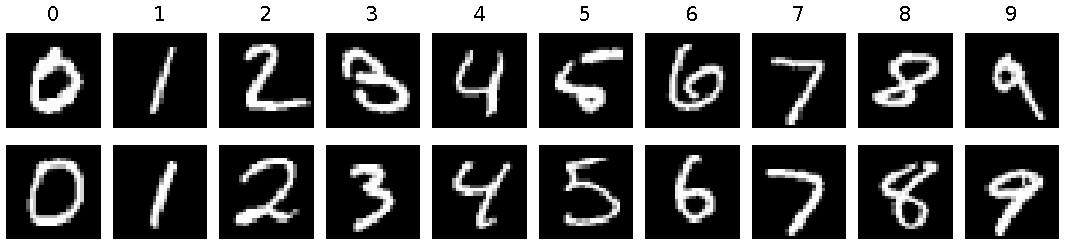
\includegraphics[width=0.96\textwidth]{mnist.pdf}
\caption{Primeras dos imágenes de cada clase en la partición oficial de prueba de MNIST. Las columnas indican las etiquetas reales; las imágenes se muestran ampliadas, sin alterar los datos originales.}
\label{fig:mnist}
\end{figure*}

\subsection{Separación de los datos}
De las 60 000 imágenes de desarrollo se separan 5 000 para validación mediante muestreo estratificado por clase y semilla 42. Las 55 000 restantes se utilizan para actualizar los pesos. Las 10 000 imágenes de prueba permanecen independientes de la selección del modelo. La Tabla~\ref{tab:particiones} resume sus funciones. La estratificación conserva aproximadamente la proporción de cada clase; no se presupone que existan exactamente mil ejemplos de cada dígito en la prueba.

\begin{table}[t]
\caption{Particiones empleadas en el proyecto}
\label{tab:particiones}
\centering
\begin{tabular}{lrl}
\hline
Partición & Imágenes & Función \\
\hline
Entrenamiento & 55 000 & Actualizar los pesos \\
Validación & 5 000 & Seleccionar la época \\
Prueba & 10 000 & Evaluación final \\
\hline
\end{tabular}
\end{table}

\subsection{Prueba sintética adicional}
Para examinar la respuesta ante cambios de presentación se seleccionan, con estratificación y semilla 123, 1 000 imágenes de la partición de prueba. A partir de ellas se generan versiones con giros de hasta aproximadamente doce grados, cambios de escala, desplazamiento sobre un lienzo de $320\times320$, variaciones de grosor e inversión de polaridad. Las transformaciones se reproducen con semillas derivadas del índice original.

Estas imágenes no constituyen otro conjunto independiente de MNIST: derivan de la prueba existente. Tampoco equivalen a fotografías reales ni a una evaluación con personas. Su función es comprobar el comportamiento del sistema ante perturbaciones sintéticas definidas antes de medir los resultados de esta comparación.

\section{Metodología}
\subsection{Preparación de la imagen}
La función \texttt{preparar} se comparte entre los ejemplos MNIST y la entrada de la aplicación. Primero corrige la orientación EXIF, compone transparencias sobre blanco y convierte a escala de grises. La mediana de los píxeles del borde permite estimar si el fondo es claro u oscuro. Se resta el fondo y se eliminan intensidades inferiores al máximo entre 18 y el 12\% de la intensidad máxima del trazo.

Luego se descartan componentes conexos muy pequeños, definidos como aquellos con menos del máximo entre dos píxeles y el 3,5\% del tamaño del componente principal. El recorte restante se ajusta proporcionalmente para que su dimensión mayor sea de 20 píxeles. Se ubica en un lienzo de $28\times28$ y se desplaza su centro de masa al centro geométrico. Una entrada sin trazo suficiente se rechaza en lugar de enviarse a la red.

Las intensidades se escalan al intervalo $[0,1]$. Dentro de la red se aplica una normalización fija:
\begin{equation}
 x' = \frac{x-0{,}1307}{0{,}3081}.
 \label{eq:norm}
\end{equation}
Estas constantes están definidas en el código; no se recalculan con la partición de prueba. El procedimiento de umbral y recorte está orientado a un dígito aislado sobre un fondo uniforme.

\subsection{Arquitectura de la red}
La red se implementa en PyTorch~\cite{pytorch2019}. Utiliza tres convoluciones de $3\times3$ con relleno de un píxel y activación ReLU. Las dos primeras se siguen de \emph{max pooling} de $2\times2$. La salida de la tercera se aplana y pasa por una capa densa de 128 neuronas, ReLU y \emph{dropout} con probabilidad 0,3. La última capa produce diez valores o \emph{logits}. La Tabla~\ref{tab:arquitectura} detalla las dimensiones; el modelo contiene \ParametrosModelo{} parámetros entrenables.

\begin{table}[t]
\caption{Arquitectura implementada}
\label{tab:arquitectura}
\centering
\begin{tabular}{ll}
\hline
Operación & Dimensión de salida \\
\hline
Entrada monocromática & $1\times28\times28$ \\
Convolución + ReLU & $24\times28\times28$ \\
Max pooling & $24\times14\times14$ \\
Convolución + ReLU & $48\times14\times14$ \\
Max pooling & $48\times7\times7$ \\
Convolución + ReLU & $64\times7\times7$ \\
Aplanado & $3136$ \\
Densa + ReLU + dropout & $128$ \\
Densa de salida & $10$ \\
\hline
\end{tabular}
\end{table}

Durante la inferencia, los logits $z_k$ se convierten a probabilidades mediante:
\begin{equation}
 p_k = \frac{\exp(z_k)}{\sum_{j=0}^{9}\exp(z_j)},\qquad
 \hat{y}=\underset{k}{\arg\max}\ p_k.
\end{equation}
El valor $p_k$ representa una estimación del modelo. No se realiza calibración de probabilidades y no debe interpretarse como una garantía de acierto.

\subsection{Entrenamiento y aumento de datos}
Se emplea entropía cruzada como función de pérdida y el optimizador AdamW~\cite{adamw}, con tasa de aprendizaje inicial de $10^{-3}$ y decaimiento de pesos de $10^{-4}$. Se procesan lotes de 256 ejemplos durante diez épocas. Un planificador coseno reduce progresivamente la tasa hacia $10^{-4}$; se invoca al finalizar cada época. La ejecución usa semilla 42 en Python, NumPy y PyTorch.

Solo los lotes de entrenamiento reciben transformaciones aleatorias. La matriz afín utiliza ángulos en $[-0{,}21,0{,}21]$ radianes, un factor de escala entre 0,88 y 1,12, un término de sesgo de hasta 0,15 y traslaciones normalizadas de hasta 0,11. La interpolación se realiza con \texttt{affine\_grid} y \texttt{grid\_sample}; por ello, los factores describen la matriz de muestreo, no un aumento exacto del tamaño visual. Además, una fracción de ejemplos mezcla el trazo con versiones suavemente engrosadas o adelgazadas.

Al final de cada época se calcula la pérdida de validación sin aumento de datos y con dropout desactivado. Se conserva el estado con la menor pérdida; en esta ejecución corresponde a la época diez. La evaluación de prueba se realiza después de seleccionar esos pesos. Las métricas y el historial se registran en archivos JSON, junto con los pesos y la versión de preprocesamiento.

\section{Implementación de la aplicación}
El sistema consta de un motor de reconocimiento en Python, un servidor HTTP local y una interfaz en HTML, CSS y JavaScript. El navegador permite dibujar mediante ratón o eventos táctiles, deshacer trazos, limpiar el lienzo y cargar imágenes PNG o JPG. El servidor prepara la imagen, ejecuta la inferencia y devuelve las probabilidades ordenadas y los píxeles procesados.

La interfaz muestra el dígito más probable, alternativas y una vista de $28\times28$. Una sección adicional presenta las métricas y la matriz de confusión. El explorador del dataset permite consultar imágenes originales, filtrar por clase y partición, identificar su índice y guardar ejemplos en PNG. Los dibujos se procesan localmente y no se envían a un servicio externo.

Los archivos principales son \texttt{motor.py}, \texttt{entrenar.py}, \texttt{servidor.py} y el directorio \texttt{web/}. El modelo anterior se conserva como referencia para la comparación y no participa en las predicciones de la aplicación actual.

\section{Resultados}
\subsection{Aprendizaje y prueba final}
La Fig.~\ref{fig:aprendizaje} presenta la evolución observada. En la última época, la exactitud de entrenamiento registrada es 98,84\% y la de validación es 99,20\%. La métrica de entrenamiento se calcula durante las actualizaciones, con transformaciones y dropout activos; no es directamente equivalente a la evaluación de validación. Por ello, una validación superior al entrenamiento no implica por sí sola un error en las particiones.

\begin{figure}[t]
\centering
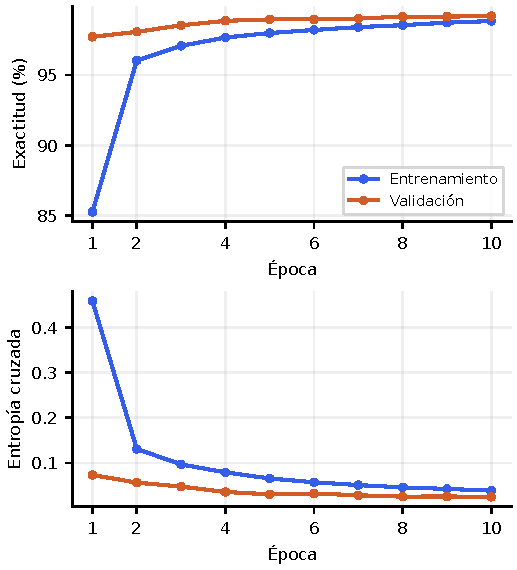
\includegraphics[width=\columnwidth]{aprendizaje.pdf}
\caption{Exactitud y pérdida por época. El entrenamiento incluye aumento de datos y dropout; la validación se evalúa sin ambos. Fuente: historial registrado por el programa.}
\label{fig:aprendizaje}
\end{figure}

En las 10 000 imágenes de prueba se obtienen 9 942 clasificaciones correctas y \NumeroErrores{} errores, equivalentes a \ExactitudPrueba\% de exactitud. El F1 macro es \FMacro. La Tabla~\ref{tab:metricas} incluye precisión, exhaustividad y F1 por clase. Para cada dígito, estas métricas se calculan a partir de verdaderos positivos, falsos positivos y falsos negativos; el promedio macro asigna igual peso a cada clase.

\begin{table}[t]
\caption{Métricas de la CNN sobre MNIST de prueba}
\label{tab:metricas}
\centering
\begin{tabular}{crrrr}
\hline
Dígito & Precisión & Exhaustividad & F1 & Soporte \\
\hline
0 & 0.9969 & 0.9990 & 0.9980 & 980 \\
1 & 0.9965 & 0.9965 & 0.9965 & 1135 \\
2 & 0.9913 & 0.9990 & 0.9952 & 1032 \\
3 & 0.9950 & 0.9941 & 0.9946 & 1010 \\
4 & 0.9909 & 0.9969 & 0.9939 & 982 \\
5 & 0.9911 & 0.9933 & 0.9922 & 892 \\
6 & 0.9979 & 0.9906 & 0.9942 & 958 \\
7 & 0.9922 & 0.9932 & 0.9927 & 1028 \\
8 & 0.9928 & 0.9938 & 0.9933 & 974 \\
9 & 0.9970 & 0.9851 & 0.9910 & 1009 \\
\hline
Macro & 0.9942 & 0.9942 & 0.9942 & 10000 \\
\hline
\end{tabular}

\end{table}

\begin{figure}[t]
\centering
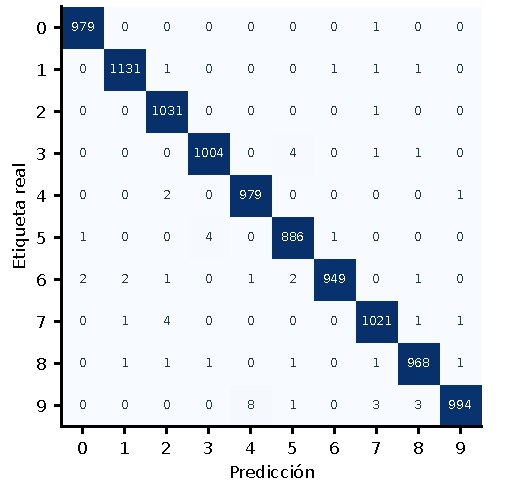
\includegraphics[width=\columnwidth]{confusion.pdf}
\caption{Matriz de confusión: filas reales y columnas predichas. Los números son conteos absolutos y el color se normaliza por fila.}
\label{fig:confusion}
\end{figure}

La matriz de la Fig.~\ref{fig:confusion} muestra que el dígito 9 presenta la menor exhaustividad, con 994 aciertos de 1 009 casos. La confusión individual más frecuente es 9 con 4, observada en ocho imágenes. La Fig.~\ref{fig:errores} presenta los primeros seis errores en el orden del conjunto de prueba, sin seleccionar manualmente los ejemplos por su apariencia.

\begin{figure}[t]
\centering
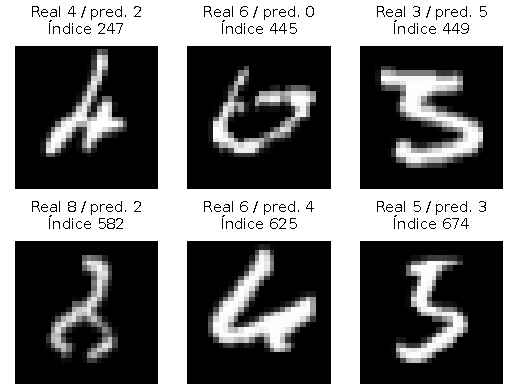
\includegraphics[width=\columnwidth]{errores.pdf}
\caption{Ejemplos de errores de la CNN, con etiqueta real, predicción e índice original de prueba. Se muestra la imagen preparada que recibe el modelo.}
\label{fig:errores}
\end{figure}

\subsection{Comparación con la implementación anterior}
La Tabla~\ref{tab:comparacion} evalúa ambos sistemas sobre las mismas entradas. El sistema anterior incluye su propia preparación a $8\times8$ y una MLP entrenada con \texttt{digits}; el actual prepara a $28\times28$ y utiliza la CNN entrenada con MNIST. La prueba sintética produce 994 aciertos de 1 000 para la CNN, frente a 175 para el sistema anterior.

\begin{table}[t]
\caption{Comparación de sistemas completos: exactitud}
\label{tab:comparacion}
\centering
\begin{tabular}{lrr}
\hline
Entradas & MLP anterior & CNN actual \\
\hline
MNIST de prueba (10 000) & 20,50\% & 99,42\% \\
Variantes sintéticas (1 000) & 17,50\% & 99,40\% \\
\hline
\end{tabular}
\end{table}

La comparación evidencia una mejora del sistema completo en el dominio MNIST. Sin embargo, cambian simultáneamente la fuente de entrenamiento, la resolución, el preprocesamiento y la arquitectura. No es una comparación controlada de MLP frente a CNN ni demuestra que toda la diferencia provenga de las convoluciones. Además, el modelo MLP fue serializado con otra versión de scikit-learn; su carga produjo advertencias de compatibilidad. Sus cifras se incluyen como diagnóstico de la implementación anterior, no como una línea base experimental definitiva.

\section{Limitaciones y reproducibilidad}
Se documenta una ejecución de entrenamiento, no un estudio de múltiples semillas. No se estimaron intervalos entre ejecuciones, tiempos de respuesta de la interfaz ni métricas de usabilidad. Las imágenes sintéticas comparten origen con MNIST y no sustituyen una evaluación con escritura de usuarios, fondos complejos o fotografías. La aplicación asume un dígito aislado y no incorpora una clase de rechazo para letras o símbolos; una imagen fuera del dominio puede recibir una predicción con alta probabilidad.

Para reproducir el proceso se instalan las dependencias del proyecto, se ejecuta \texttt{python entrenar.py --epocas 10} y después \texttt{python evaluar.py}. La comparación adicional se obtiene con \texttt{python evaluar\_robustez.py}. La ejecución registrada utilizó Python 3.9.6 y PyTorch 2.8.0 en CPU. El registro marca 122,5 segundos desde el inicio del bucle de entrenamiento hasta la evaluación final; excluye descarga y preparación de datos, y no representa una medición comparativa de rendimiento. Otras versiones o dispositivos pueden producir diferencias numéricas.

Como trabajo futuro se propone recopilar, con consentimiento, un conjunto independiente de dibujos reales, evaluar una MLP entrenada con las mismas particiones que la CNN y estudiar calibración o rechazo de entradas desconocidas. Estas tareas no forman parte de los resultados presentados.

\section{Conclusiones}
Se desarrolló una aplicación funcional para reconocer dígitos mediante una CNN e interacción web local. La preparación compartida, el uso de imágenes de mayor resolución y el entrenamiento con transformaciones permiten obtener 99,42\% de exactitud en MNIST de prueba. La integración conserva trazabilidad mediante métricas, pesos, semillas y un explorador de los datos. Los resultados apoyan su uso como proyecto académico de clasificación de dígitos aislados, mientras que la eficacia sobre escritura real requiere una evaluación adicional.

\bibliographystyle{IEEEtran}
\bibliography{referencias}
\end{document}
